In the following set of experiments with the Blackbird dataset, we split the data into in/out-of-distribution by trajectory. Recall that the datasets consists of 163 unique flight sequences, and each sequence follows one of seventeen trajectories. We select four challenging trajectories as OOD and exclude all their sequences from the training data, details of the split available in \cref{app:blkbrd_split}. 

As we will see in the results, with this split the models can generalize well to the OOD inputs, despite the fact that the probability of those inputs is zero under the training distribution. This provides a different setting from the one we saw in the last section, where model errors increased for the OOD data.

This section will follow the same structure as the previous one, but will proceed faster and focus on validating the key findings. 

\subsection{C-RNN analysis}

\begin{table*}[h]
\centering
    \begin{tabular}{c  c  c   c  c }  
        \toprule
        Split & MAE & NLL & $\mathcal{A}$ & $\mathcal{E}$\\
        \midrule
        Test & 0.3(0.29, 0.31) & 0.3(0.27, 0.33) & 0.31(0.3, 0.32) &  -6.1\\
        OOD  &  0.27(0.25, 0.29) &  0.13(0.03, 0.22) & 0.28(0.27, 0.29)&  -6.2\\
        \midrule
    \end{tabular}
    \caption{Blackbird(1) C-RNN performance.}
    \label{tbl:bb1_CRNN}
\end{table*}

% \begin{figure}[h]
%   \centering
  
%   \begin{subfigure}[b]{\textwidth}
%     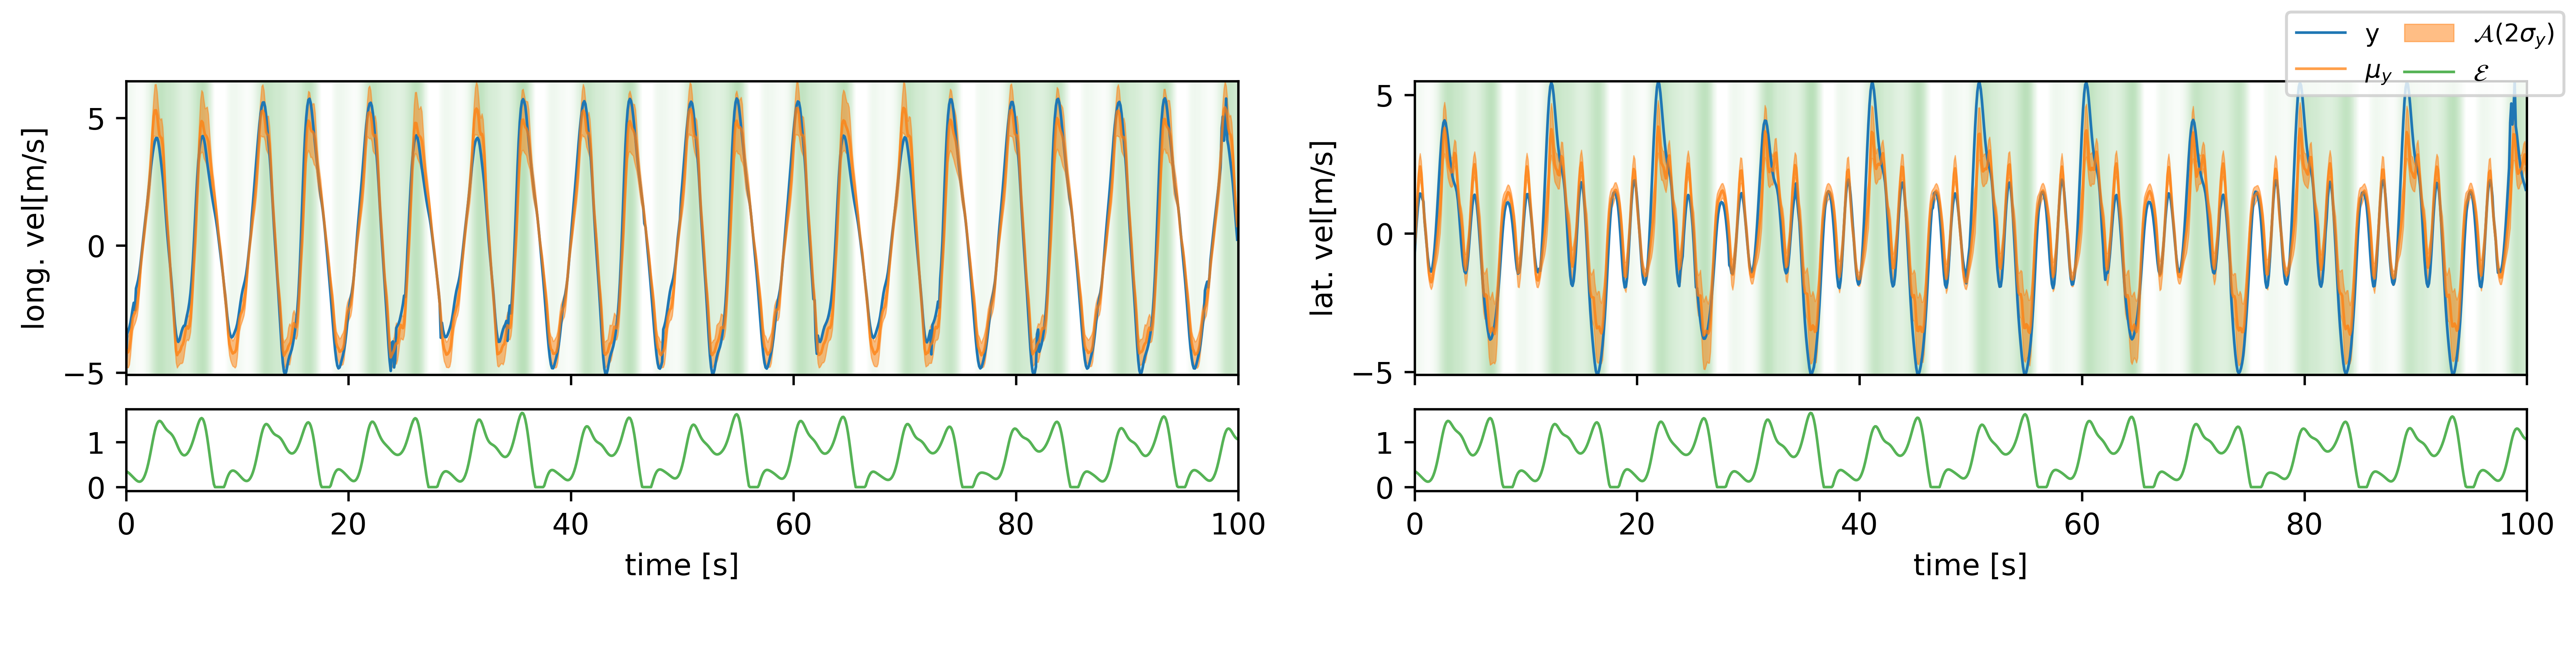
\includegraphics[width=\textwidth]{Experiments/figs/bb1_test.png}
%     \caption{Test}
%   \end{subfigure}
  
%   \begin{subfigure}[b]{\textwidth}
%     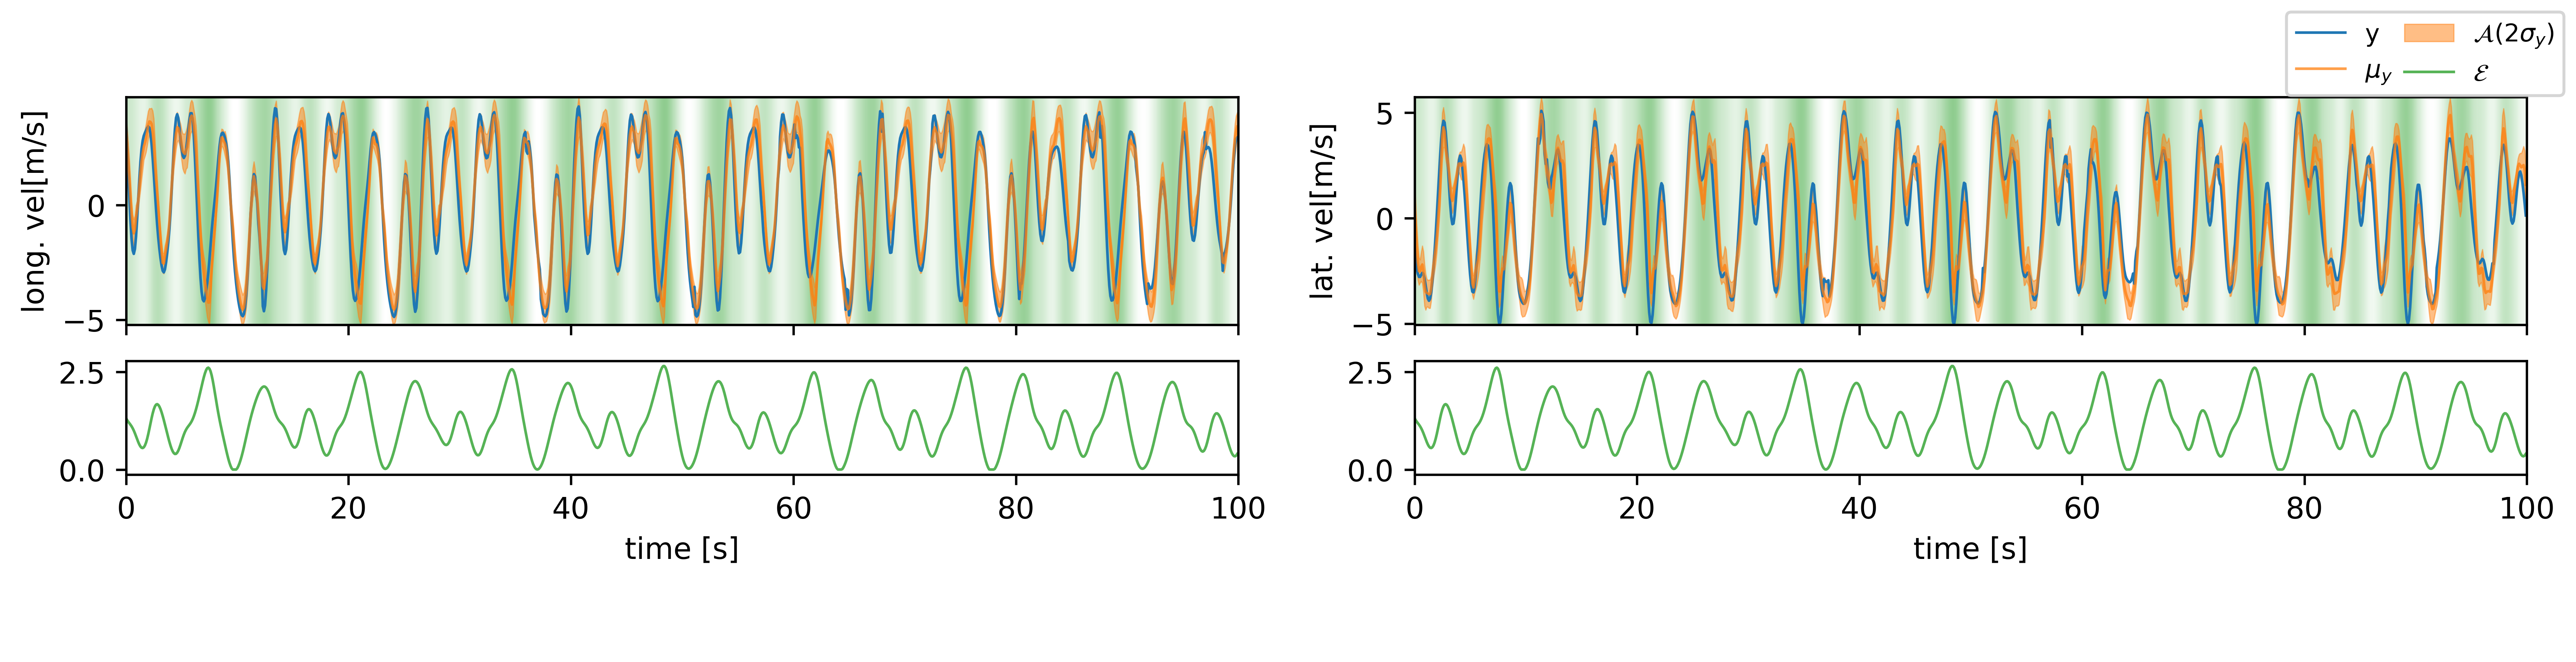
\includegraphics[width=\textwidth]{Experiments/figs/bb1_ood.png}
%     \caption{OOD}
%   \end{subfigure}
  
%   \caption{Blackbird(1) prediction plots for C-RNN.}
%   \label{fig:bb1_run}
% \end{figure}

\Cref{fig:bb1_run} shows a flight sequence with the model predictions for a test and an OOD input. We can see from the plots that the model behavior and quality of predictions is quite similar for the two sequences. In \cref{tbl:bb1_CRNN} we can see that the performance of C-RNN is similar for the two splits.

This is a tricky setting, since the model's errors are not correlated with the input being in or out-distribution. Recall that being out-of-distribution simply means the probability of the input is zero under the training distribution, this does not automatically imply that the model won't be able to generalize to some of those inputs. In fact we can see here that the model generalizes quite well, even giving a lower NLL of 0.13 for the OOD split, compared to 0.3 over the test split. In this case, we would not want our epistemic uncertainty to be high for OOD inputs in general, but rather to correlate with the errors. 
Fortunately, we can already see in \cref{tbl:bb1_CRNN} that the epistemic uncertainty on average is roughly the same for both splits. 

This setting shows how metrics such as AUROC which are widely used in works for OOD detection~\citep{liang2017enhancing, hein2019relu, lee2017training} are only meaningful if we assume that the model performs poorly on the OOD data we have. We have shown in the previous section that C-RNN's epistemic uncertainty estimates did an excellent job separating the in/out-of-distribution points with an AUROC of 0.97. In this setting, our C-RNN has an AUROC of 0.46, which is close to random behavior. This is a desirable result in this case, since there is no reason for the uncertainty to be higher in general on the OOD inputs if the errors are not.


\begin{table*}[h]
\centering
    \begin{tabular}{l l c c c c}  
        \toprule
        U. & Split & \multicolumn{2}{c}{MAE} & \multicolumn{2}{c}{$Zs$}\\
        \midrule
        & & $\rho \uparrow$ & $r \uparrow$ & $\rho \uparrow$ & $r \uparrow$ \\
        \multirow{3}{*}{$\mathcal{A}$} 
            & Test     & 0.81(0.81, 0.81) & 0.81(0.78, 0.84) & - & - \\  
            & OOD      & 0.86(0.9, 0.81) & 0.88(0.89, 0.87) & - & - \\  
            & Test+OOD & 0.84(0.87, 0.80) & 0.86(0.86, 0.86) & - & - \\ 

        \midrule
        \multirow{3}{*}{$\mathcal{E}$} 
            & Test     & 0.88  & 0.86 &  0.31  & 0.41 \\  
            & OOD      & 0.90 & 0.89 &  0.51 & 0.64 \\
            & Test+OOD & 0.88 & 0.86 &  0.44 & 0.57 \\ 

        \toprule
    \end{tabular}
    \caption[Blackbird(1) error-uncertainty correlation for C-RNN]{Blackbird(1) Pearson $\rho$ and Spearman $r$ correlations between the uncertainties and error scores for C-RNN.}
    \label{tbl:bb1_corr}
\end{table*}

Our best test for quality of the uncertainty estimates in this case is their correlation with the errors. \Cref{tbl:bb1_corr} shows the correlations between our error scores and uncertainties.  Here we note that both the aleatoric and epistemic uncertainty correlate highly with the MAE. The aleatoric uncertainty has a Pearson correlation of 0.84 with the MAE, and the epistemic uncertainty has a correlation of 0.88 with the MAE. 

The high correlation of the epistemic uncertainty with the errors is good news, given that we are in the context where OOD data have the same MAE as the in-distribution data. However, the strong correlation of the aleatoric and epistemic uncertainty with the MAE suggests that they may be giving the same information. Indeed we find that the Pearson correlation between the epistemic and aleatoric uncertainty to be 0.95. Thus in the particular setting here we see redundancy between our two uncertainty estimates, but on a positive note they both correlate with the errors well, and we at least don't see our model assign overly high uncertainties to the OOD inputs. Recall that in the Revs dataset, C-RNN assigned much larger uncertainties to the OOD data with an average -0.25 epistemic uncertainty for the OOD data and an average -4.6 epistemic uncertainty to the test data. Thus on a positive note, the model is flexible enough to cope with both situations. 

\begin{figure}[htbp]
  \centering
    \begin{subfigure}[b]{\textwidth}
        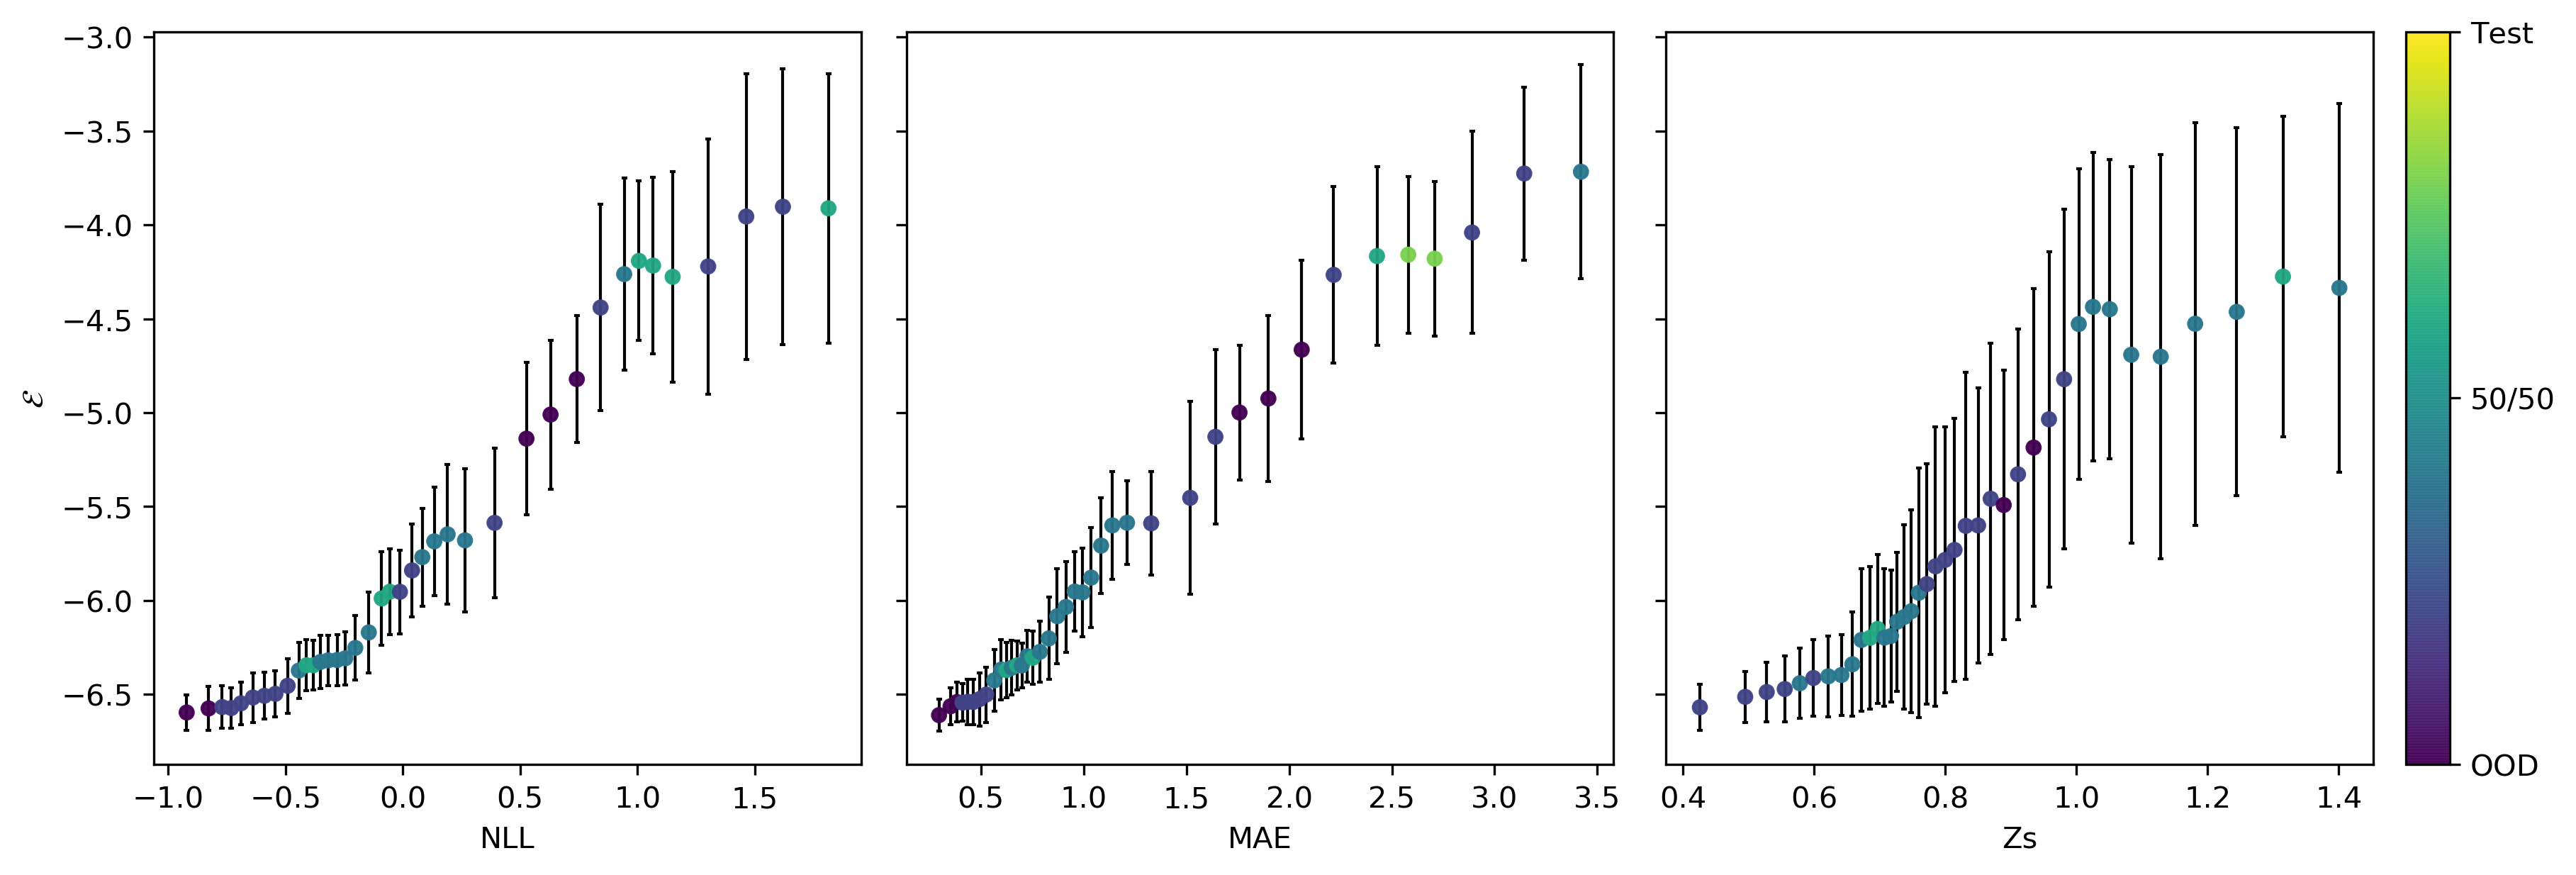
\includegraphics[width=\textwidth]{Experiments/figs/binned/bb1_crnn_epistemic.png}
        \caption{Binned diagonal plots for the epistemic uncertainty.}
    \end{subfigure}
    
    \begin{subfigure}[b]{\textwidth}
        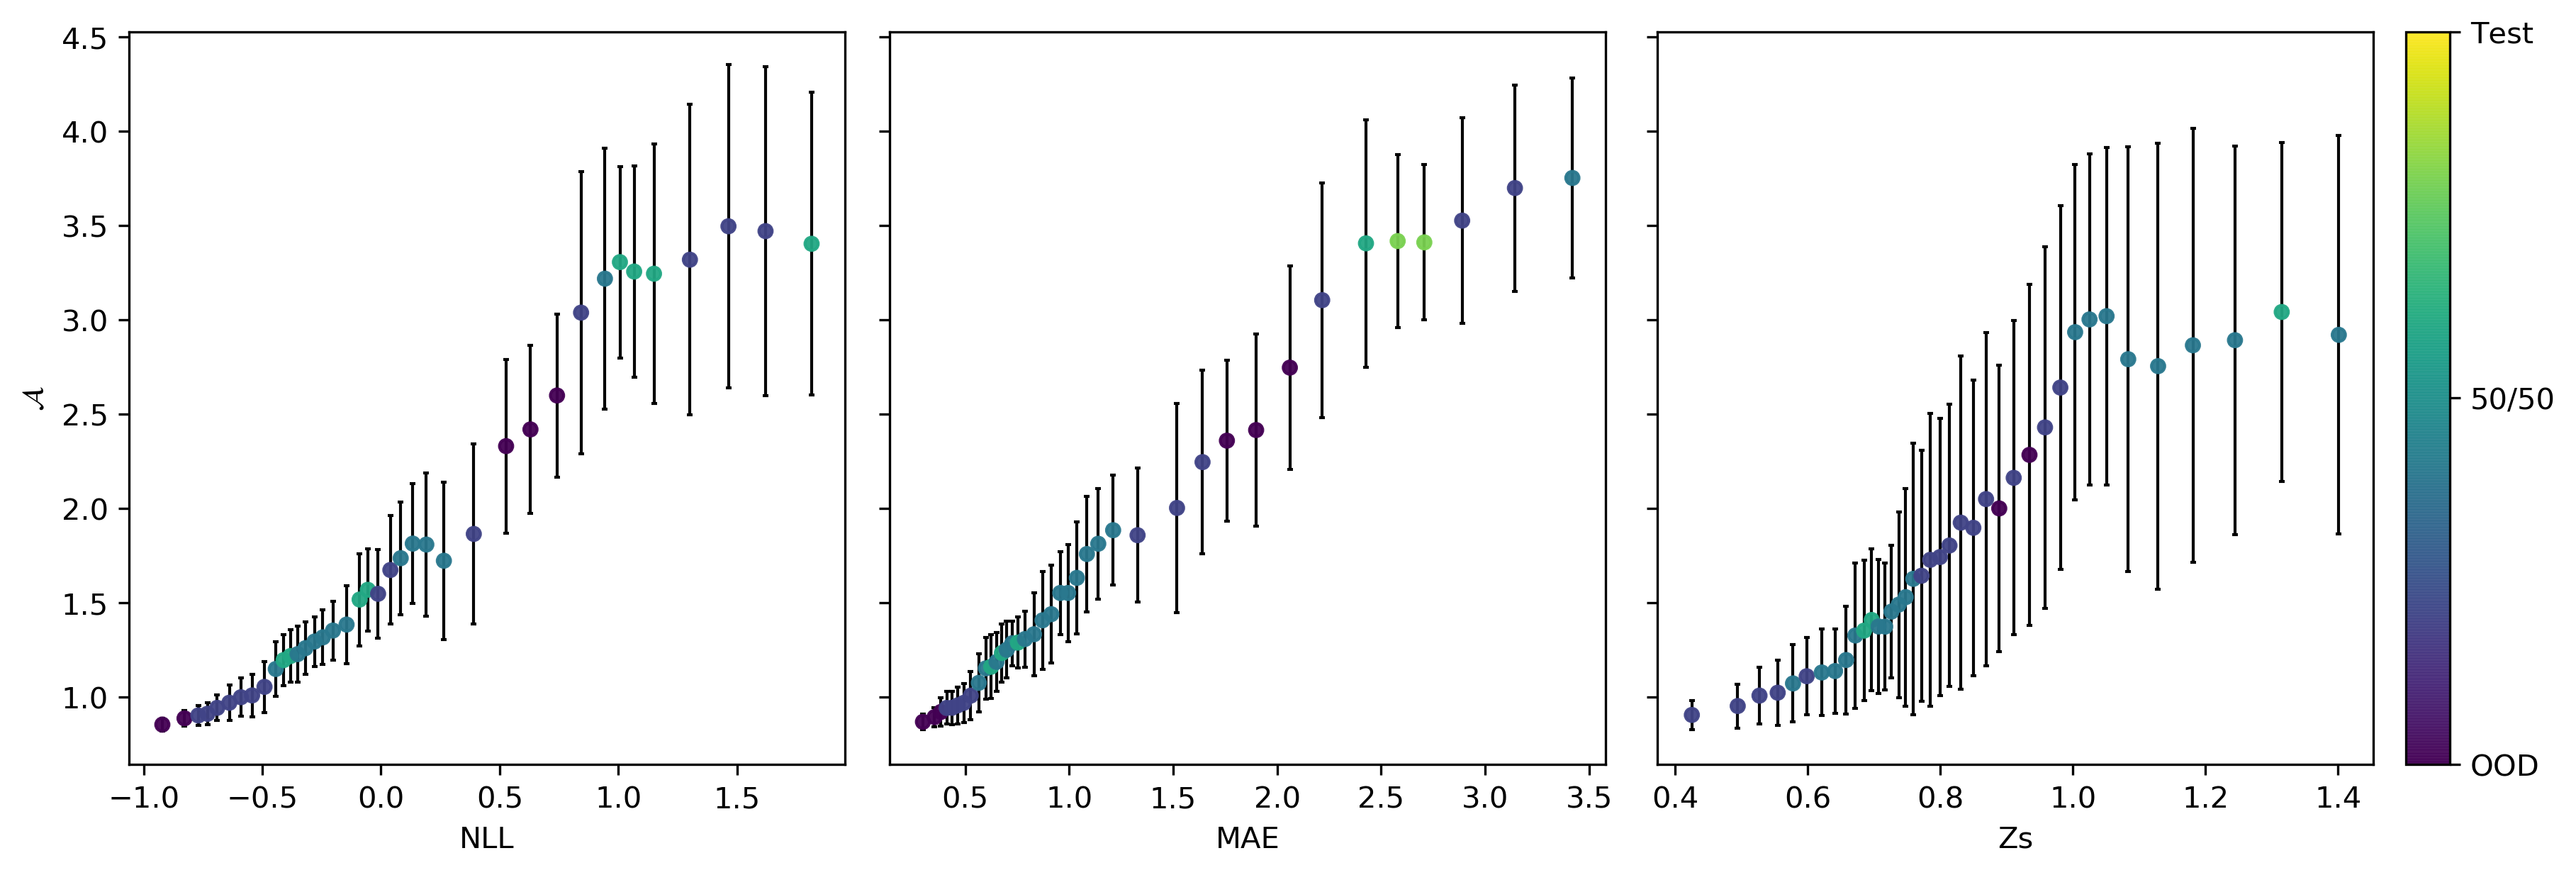
\includegraphics[width=\textwidth]{Experiments/figs/binned/bb1_crnn_aleatoric.png}
        \caption{Binned diagonal plots for the aleatoric uncertainty.}
  \end{subfigure}
    \caption[Blackbird(1) error-uncertainty diagonal plots for C-RNN]{Blackbird(1) binned diagonal plots of the  uncertainty vs error scores(NLL, MAE, Z-score) over the combined splits(Test+OOD). The marker color denotes the ratio of test to OOD points in the bin. }
    \label{fig:bb1_uncertainty_corr}
\end{figure}

\Cref{fig:bb1_uncertainty_corr} shows the binned diagonal plots between our errors and uncertainties. We can see that in this case, the two uncertainties behave similarly with respect to the errors. Unlike the Revs experiment (\cref{sec:revs_results}) We do not see a clear separation of in/out-of-distribution points, the bins seem largely mixed. Overall, both uncertainties correlate with the errors.  
In the next section we will look at how MC dropout behaves, then we will follow with the key findings and a comparison of the approaches.


\clearpage
\subsection{MC dropout analysis}

\begin{table*}[ht]
\centering
    \begin{tabular}{c  c  c   c  c }  
        \toprule
        Split & MAE & NLL & $\mathcal{A}$ & $\mathcal{E}$\\
        \midrule
        Test & 0.26(0.26, 0.27) & 0.2(0.19, 0.22) & 0.41(0.42, 0.41) &  0.26(0.27, 0.26)\\
        OOD  &  0.28(0.26, 0.29) &  0.23(0.21, 0.26) & 0.4(0.41, 0.39)&  0.24(0.25, 0.24)\\
        \midrule
    \end{tabular}
    \caption{Blackbird(1) MC dropout performance.}
    \label{tbl:bb1_dropout}
\end{table*}

% \begin{figure}[ht]
%   \centering
  
%   \begin{subfigure}[b]{\textwidth}
%     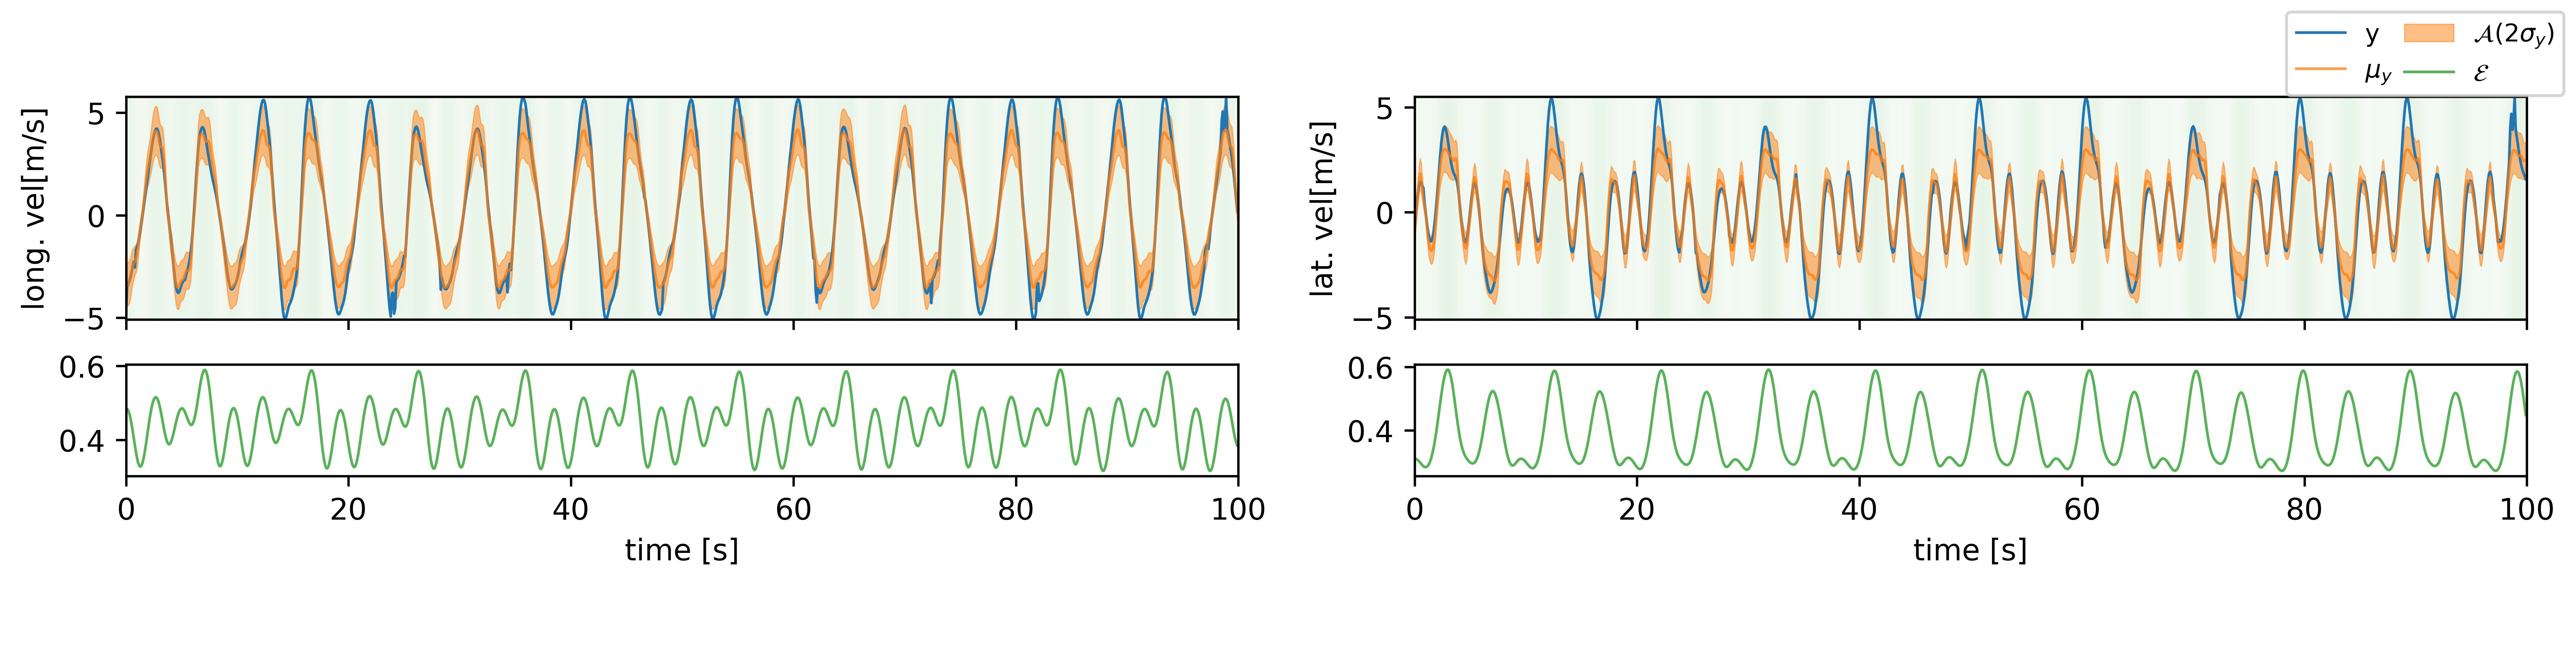
\includegraphics[width=\textwidth]{Experiments/figs/bb1_dropout_test.png}
%     \caption{Test}
%   \end{subfigure}
  
%   \begin{subfigure}[b]{\textwidth}
%     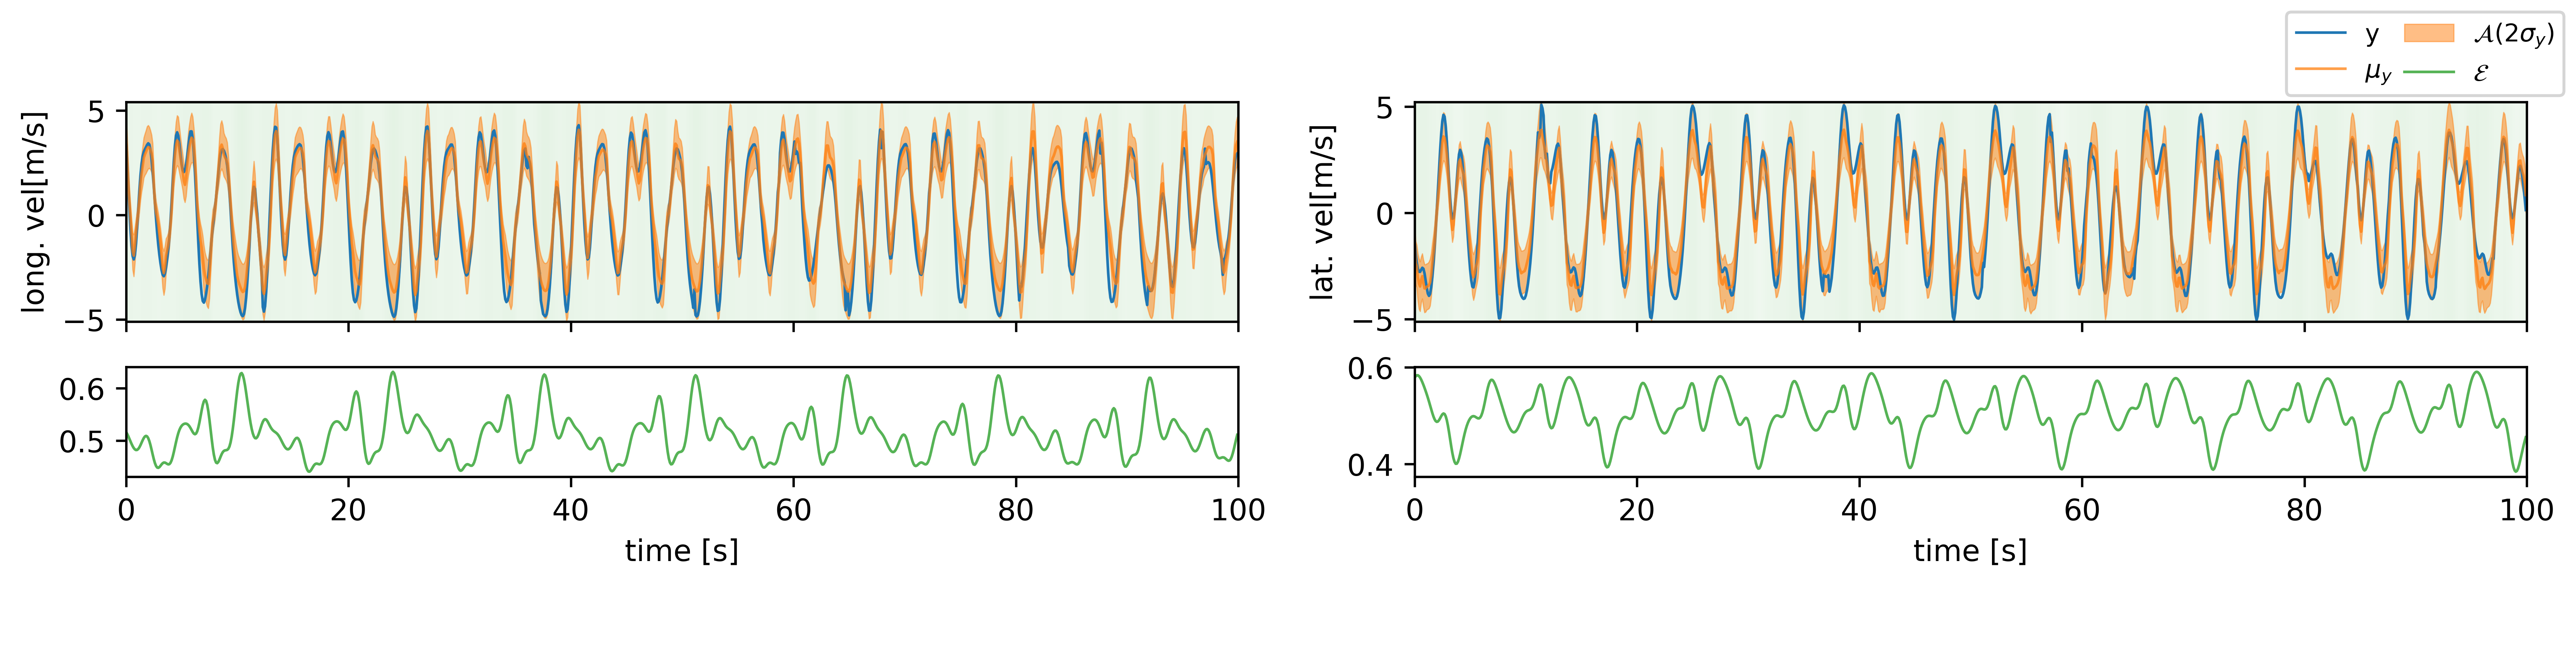
\includegraphics[width=\textwidth]{Experiments/figs/bb1_dropout_ood.png}
%     \caption{OOD}
%   \end{subfigure}
  
%   \caption{Blackbird(1) prediction plots for MC dropout.}
%   \label{fig:bb1_dropout_run}
% \end{figure}

\Cref{fig:bb1_dropout_run} shows a flight sequence with the model predictions for a test and an OOD sequence for the MC dropout model. Again we can see from the plots that the model behavior and quality of predictions is quite similar for the two sequences. \Cref{tbl:bb1_dropout} contains the basic performance metrics for the MC dropout model, and again we see that the model performance is similar for the test and OOD splits.

In terms of discriminating between the two splits, we can already see in \cref{tbl:bb1_dropout} that the uncertainties are on average the same for the test and OOD split. In fact the AUROC for MC dropout is 0.46 using the epistemic uncertainty. We show the correlation between the uncertainties and errors for MC dropout in \cref{tbl:bb1_dropout_corr} . We see similar trends to those of C-RNN in \cref{tbl:bb1_corr}, with both the aleatoric and epistemic uncertainties highly correlated with the MAE for all splits. Finally we compute the Pearson correlation between the epistemic and aleatoric uncertainties for the dropout model and get a 0.96 coefficient, showing that the uncertainties are also highly correlated for MC dropout. In the next subsection we will distill the key findings from the previous results and contrast the behavior of C-RNN and MC dropout in this setting.

\begin{table*}[ht]
\centering
    \begin{tabular}{l l c c c c}  
        \toprule
        U. & Split & \multicolumn{2}{c}{MAE} & \multicolumn{2}{c}{$Zs$}\\
        \midrule
        & & $\rho \uparrow$ & $r \uparrow$ & $\rho \uparrow$ & $r \uparrow$ \\
        \multirow{3}{*}{$\mathcal{A}$} 
            & Test     & 0.78(0.80, 0.76) & 0.82(0.82, 0.82) & - & - \\  
            & OOD      & 0.79(0.82, 0.75) & 0.85(0.85, 0.84) & - & - \\  
            & Test+OOD & 0.79(0.82, 0.76) & 0.83(0.84, 0.82) & - & - \\ 

        \midrule
        \multirow{3}{*}{$\mathcal{E}$} 
            & Test     & 0.76(0.76, 0.75) & 0.81(0.8, 0.81) &  0.42(0.42, 41)  & 0.45(0.43, 0.47) \\  
            & OOD      & 0.77(0.82, 0.72) & 0.83(0.84, 0.82) &  0.4(0.44, 0.35) & 0.45(0.49, 0.41) \\
            & Test+OOD & 0.76(0.79, 0.73) & 0.82(0.82, 0.81) &  0.4(0.43, 0.36) & 0.45(0.47, 0.42) \\ 

        \toprule
    \end{tabular}
    \caption[Blackbird(1) error-uncertainty correlations for MC dropout]{Blackbird(1) Pearson $\rho$ and Spearman $r$ correlations between the uncertainties and error scores for MC dropout.}
    \label{tbl:bb1_dropout_corr}
\end{table*}

\begin{figure}[htbp]
  \centering
    \begin{subfigure}[b]{\textwidth}
        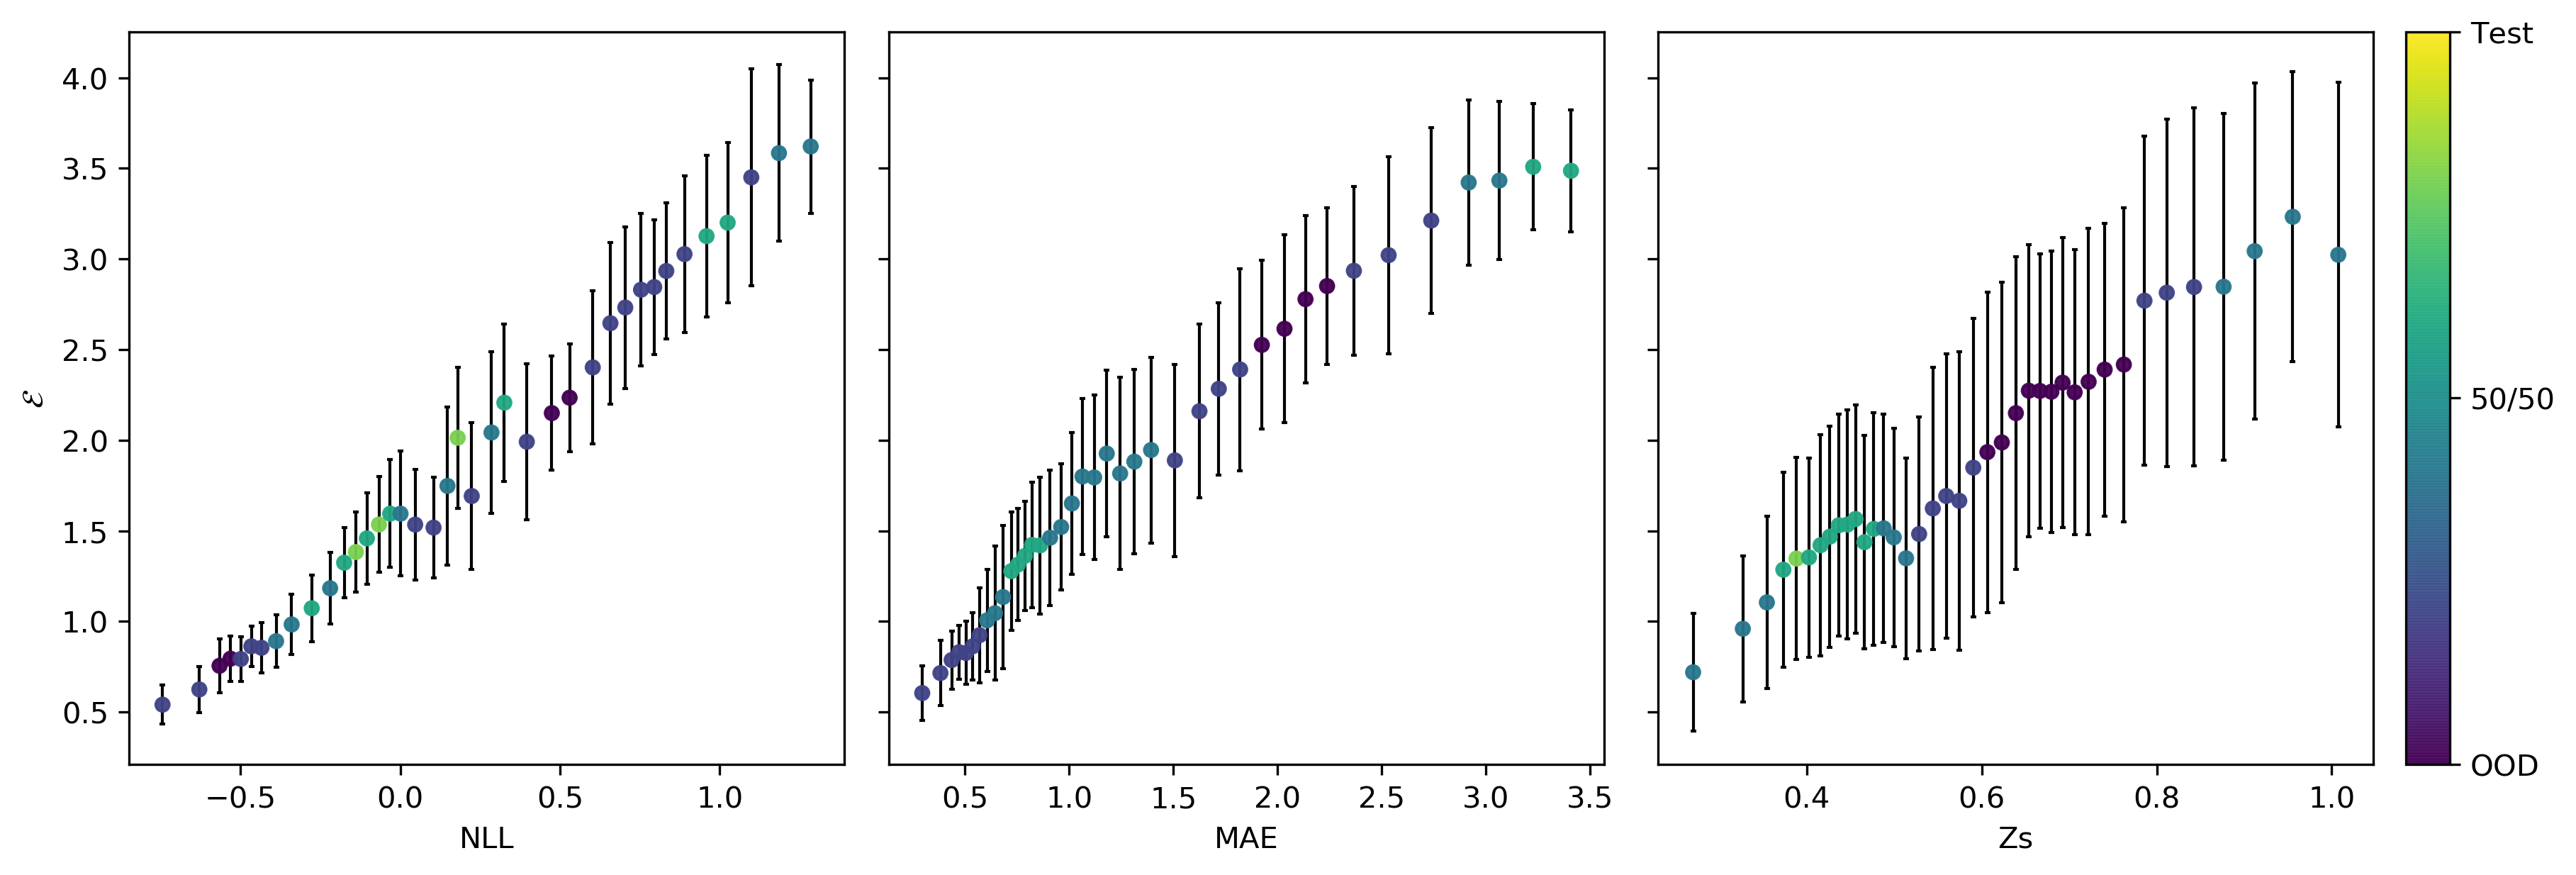
\includegraphics[width=\textwidth]{Experiments/figs/binned/bb1_dropout_epistemic.png}
        \caption{Binned diagonal plots for the epistemic uncertainty.}
    \end{subfigure}
    
    \begin{subfigure}[b]{\textwidth}
        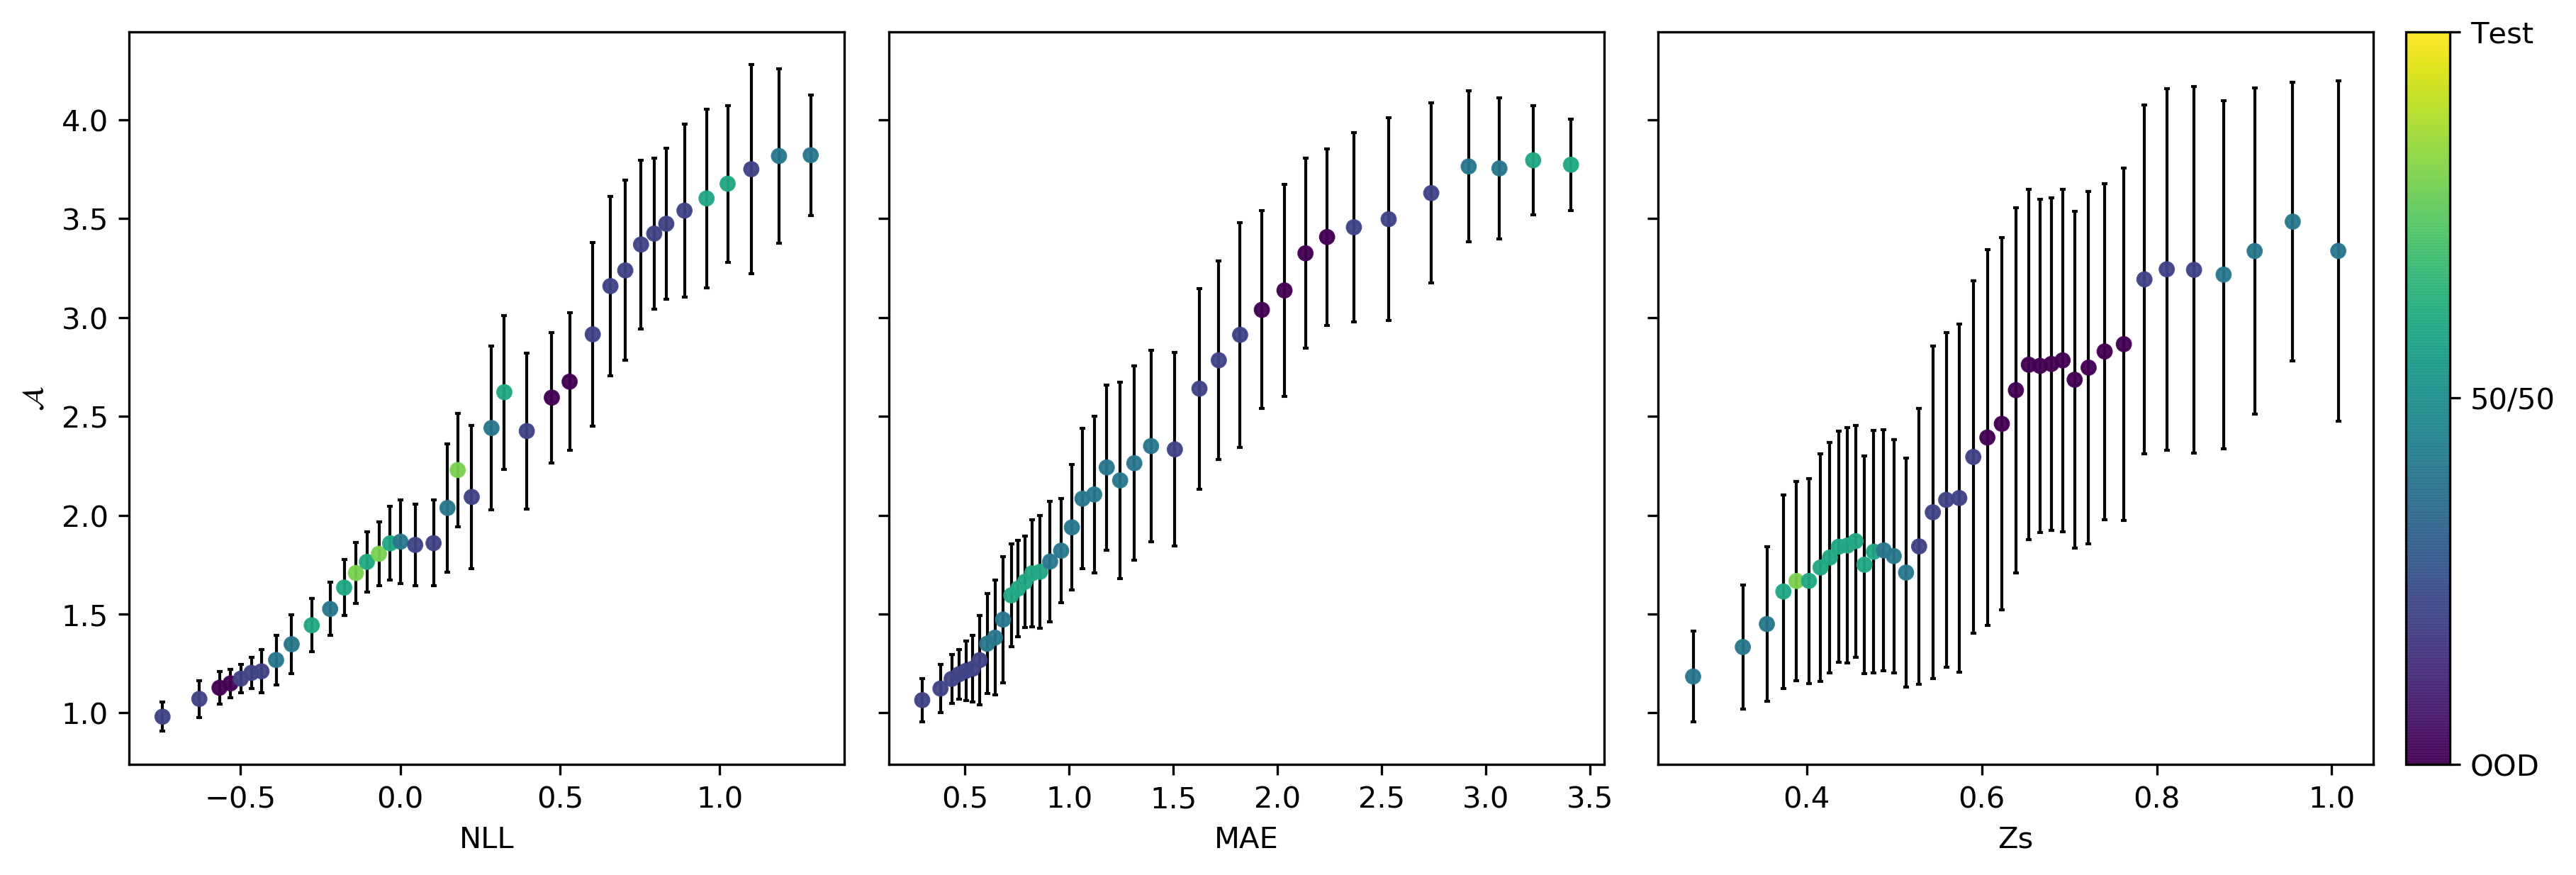
\includegraphics[width=\textwidth]{Experiments/figs/binned/bb1_dropout_aleatoric.png}
        \caption{Binned diagonal plots for the aleatoric uncertainty.}
  \end{subfigure}
    \caption[Blackbird(1) error-uncertainty diagonal plots for MC dropout]{Blackbird(1) binned diagonal plots of the  uncertainty vs error scores(NLL, MAE, Z-score) over the combined splits(Test+OOD). The marker color denotes the ratio of test to OOD points in the bin. }
    \label{fig:bb1_dropout_uncertainty_corr}
\end{figure}

\Cref{fig:bb1_dropout_uncertainty_corr} shows the binned diagonal plots for the errors versus uncertainty for MC dropout. The general patterns for the error-uncertainty correlations here are the same as for the C-RNN model. We see that both uncertainties behave similarly, the in/out-of-distribution points seem mixed within the bins, and both uncertainties correlate with the errors. 



\subsection{Key findings}

Recall that a key property of how we split the Blackbird dataset for this experiment was that the models could generalize to the OOD data. The key findings for our first split of Blackbird

\begin{itemize}
    \item Both models generalize well to the OOD data.
    \item Both models' epistemic uncertainty is on average equal for the test and OOD data.
    \item Both model show a high correlation between the MAE and the uncertainties.
    \item Both models a high correlation between their epistemic and aleatoric uncertainty estimates. 
\end{itemize}{}

In short, C-RNN and MC dropout qualitatively behave the same here. \Cref{tbl:bb1_comparison} shows the key results for both models. We can see that the performance of both models is close with the NLL being equal. For the epistemic uncertainty, we can see the C-RNN's epistemic uncertainty correlates slightly better with the MAE, giving a Pearson coefficient of 0.88 versus 0.76 for MC dropout. The correlation with the Z-score is roughly the same for both models. Also as we have mentioned both models show high correlation between their epistemic and aleatoric uncertainty estimate(C-RNN: 0.95, MC dropout: 0.96).  


\begin{table*}[h]
\centering
    \begin{tabular}{l l c c c c c}  
        \toprule
        Model & split & MAE & NLL & $\rho$(MAE vs $\mathcal{E}$) &
        $\rho$(Z-score vs $\mathcal{E}$) & AUROC($\mathcal{E}$)\\
        \midrule
        \multirow{3}{*}{C-RNN} 
            & Test     & 0.3  & 0.3  & 0.88  & 0.31 & - \\  
            & OOD      & 0.27 & 0.13 & 0.90  & 0.51 & -\\  
            & Test+OOD & 0.28 & 0.21 & 0.88  & 0.44 & 0.46\\ 

        \midrule
        \multirow{3}{*}{MC dropout} 
            & Test     & 0.26 & 0.2  & 0.76  & 0.42 & - \\  
            & OOD      & 0.28 & 0.23 & 0.77  & 0.4 & -\\  
            & Test+OOD & 0.27 & 0.21 & 0.76  & 0.4 & 0.46\\ 

        \toprule
    \end{tabular}
    \caption{Blackbird(1) key results for comparison of C-RNN and MC dropout.}
    \label{tbl:bb1_comparison}
\end{table*}


To conclude, we have created a situation where OOD inputs do not have higher errors than in-distribution inputs. This should be a challenging setting for C-RNN, as we have seen on the Revs dataset(\cref{sec:revs_results}), it consistently gave higher uncertainty to OOD inputs with an AUROC of 0.97. In this setting, this behavior would lead the epistemic uncertainty to be misleading. However, C-RNN handles the situation well, and preforms on par with MC dropout. In the coming section we will show a different set of experiments with the Blackbird dataset, where we chose a different in/out-of-distribution split. 
